\section{Auswertung}

Zunächst muss im Versuch die Winkelrichtgröße $D$ und das
das Eigenttägheitsmoment der Drillachse $I_D$ bestimmt werden.
Anschließend die Trägheitsmoment einer Kugel und eines Zylinder (\emph{grau}).
Abschließend noch die Trägheitsmomente von einer Holzpuppe in zwei verschieden Positionen.
Da das Trägheitsmoment nicht direkt gemessen werden kann wurden immer 
die Schwingungsdauer $T$ von $5$ Schwingungen gemessen.

\subsection{Bestimmung der Winkelrichtröße $D$}

Die Winkelrichtgröße $D$ kann auf zwei verschiedene Wege bestimmt werden.
Zum einem durch eine passive und zum andern durch eien  dynamische Methode.
Beide Methoden werden im Anschluss genauer erklärt und verwendet.
Nach der Bestimmung der beiden Winkelrichtgrößen $D_{passiv}$ und $D_{dynam}$
werden diese verglichen.


\subsubsection{Passive Methode}

Die passive oder auch als statisch bezeichnete Methothde wurden mittels einem Drehmoment (gemessen mit einer Federwaage) ausgelenkt.
Wichtig dabei ist das die Federwaage immer orthogonal zum Radius steht.
Denn das Drehmoment errechnet sich mit $\vec{M}=\vec{r}\times\vec{F}$, durch 
eine orthogonale Stellung von $\vec{r}$ und $\vec{F}$ kann mit den Beträgen 
gerechnet werden und es ergibt sich der Zusammenhang $M=rF$. 
Im Versuch wurden folgende Werte bestimmt:


\begin{table}
\centering
\caption{Messung der Kraft für eine Auslenkung}
\label{tab: winkelricht}
\renewcommand{\arraystretch}{1.2}
\begin{tabular}{lcr}
	\toprule
	Abstand in $\si{\meter}$ & Winkel in $\mathrm{rad}$ & Kraft in $\si{\newton}$ \\
	\midrule
	$\num{1.01e-1}$ & $\frac{\pi}{6}$ & $\num{1.40e-1}$ \\
	$\num{1.01e-1}$ & $\frac{\pi}{3}$ & $\num{2.40e-1}$ \\
	$\num{1.01e-1}$ & $\frac{\pi}{2}$ & $\num{3.20e-1}$ \\
	$\num{1.01e-1}$ & $\frac{2\pi}{3}$ & $\num{4.60e-1}$ \\
	$\num{1.58e-1}$ & $\frac{\pi}{6}$ & $\num{6e-2}$ \\
	$\num{1.58e-1}$ & $\frac{\pi}{3}$ & $\num{1.2e-1}$ \\
	$\num{1.58e-1}$ & $\frac{\pi}{2}$ & $\num{2.20e-1}$ \\
	$\num{1.58e-1}$ & $\frac{2\pi}{3}$ & $\num{3e-1}$ \\
	$\num{2.41e-1}$ & $\frac{\pi}{6}$ & $\num{2.00e-2}$ \\
	$\num{2.41e-1}$ & $\frac{\pi}{3}$ & $\num{8.00e-2}$ \\
	$\num{2.41e-1}$ & $\frac{\pi}{2}$ & $\num{1.2e-1}$ \\
	$\num{2.41e-1}$ & $\frac{2\pi}{3}$ & $\num{2.00e-2}$ \\
	\bottomrule
\end{tabular}
\end{table}

Mit dem Zusammenhang

\begin{equation*}
D=\frac{M}{\phi}=\frac{Fr}{\phi}
\end{equation*}

ergibt sich dann für jede einzelne der $n$ Messungen ergibt sich dann ein Wert für die Winkelrichtgröße.
Diese wurden anschließend durch

\begin{equation}
\label{eq:mittel}
\bar{x}=\frac{1}{n}\sum_{i=1}x_i
\end{equation}

gemittelt, mit der dazugehörigen Abweichung

\begin{equation}
\label{eq:stand_ab}
\bar{\sigma}_{\bar{x}}=\sqrt{\frac{1}{n(n-1)}\sum_{i=1}^{n}(x_i-\bar{x})^2}.
\end{equation}

Es ergibt sich dann für damit für die Winkelrichtgröße der Wert:

\begin{equation}
\label{eq:winkel_passiv}
D_{passiv}=\left(\num{2.03e-2} \pm \num{1.22e-3}\right)\si{\newton\meter}
\end{equation}

\subsubsection{Dynamische Methode}

Bei der dynamischen Methode wurden die Schwingungsdauer von zwei kleinen Zylindern ($m_1$ und $m_2$) die symetrisch zum Mittelpunktes
eines Stabes befestigt waren gemmessen. Durch Verschiebung der Massen ergab sich eine Vielzahl von Messwerten, die im Anhang eingesehn
werden können.
Diese wurden anschließend gemittelt mit \eqref{eq:mittel} und \eqref{eq:stand_ab}.

\begin{table}
\centering
\caption{Gemittelte Schwingungsdauer für die dynamische Methode}
\label{tab: winkel_dynamisc}
%\renewcommand{\arraystretch}{1.2}
\begin{tabular}{lr}
	\toprule
	$\bar{T}$ in $\si{\per\second}$ &  $\sigma_{\bar{T}}$ in $\si{\per\second}$ \\
	\midrule
	\num{2.52} & \num{6.43e-3} \\
	\num{3.23} & \num{9.16e-3} \\
	\num{3.65} & \num{5.89e-3} \\
	\num{4.08} & \num{3.57e-3} \\
	\num{4.56} & \num{6.82e-3} \\
	\num{5.09} & \num{2.83e-2} \\
	\num{5.56} & \num{3.33e-2} \\
	\num{6.05} & \num{1.07e-2} \\
	\num{6.59} & \num{8.64e-3} \\
	\num{7.07} & \num{3.31e-3} \\
	\bottomrule
\end{tabular}
\end{table}

Mit den Schwingungsdauern und dem Gesetzt:

\begin{equation*}
T=2\pi\sqrt{\frac{I}{D}} \quad \Leftrightarrow \quad I=\frac{T^2 D}{4\pi^2}
\end{equation*}

Da die Massen von der Drehachse verschoben waren, macht man sich den Satz von Steiner \eqref{eq: steiner} zu nutze und erhält den Zusammenhang:

\begin{equation}
\label{eq:gerade}
\frac{T^2D}{4\pi^2}=I_s+ma^2\quad \Leftrightarrow \quad T^2=\frac{I_s 4\pi^2}{D}+\frac{4m_g\pi^2}{D}a^2
\end{equation}

Dabei sei $m_g=m_1+m_2$.
Offensichtlich ergibt sich eine Geradengleichung, die mit Linearer Regression angenährt werden kann.
Dazu verwendet man aus der Regressionsrechnung.

Für die Steigung $m$ ergibt sich

\begin{equation*}
m=\frac{\bar{xy}-\bar{x}\bar{y}}{\bar{x^2}-\bar{x}^2}
\end{equation*}

,mit dem dazugehörigen Fehler

\begin{equation*}
\sigma_m=\sqrt{\frac{\sigma^2}{N(\bar{x^2}-\bar{x}^2)}}.
\end{equation*}

Nach Ausführung der Regressionrechnung erhält man als Wert
\begin{equation}
\label{eq: steigung}
m=\left(\num{741.2}\pm\num{3.4}\right) \si{\kilogram\per\newton\meter}
\end{equation}

Da es sich bei \eqref{eq:gerade} um eine Gerade handelt muss gelten:

\begin{equation*}
m=\frac{4m_g\pi^2}{D}
\end{equation*}

Damit kann die Winkelrichtgröße dynamisch bestimmt werden

\begin{equation*}
D=\frac{4m_g\pi^2}{m}.
\end{equation*}

Er ergibt sich:

\begin{equation}
\label{winkelrichtgroesse_dynamisch}
D_{dynam}=\left(\num{2.38e-2} \pm \num{1.10e-4}\right)\si{\newton\meter}
\end{equation}

Da die Abweichung von $D_{dynam}$ kleiner ist als von $D_{passiv}$ wird 
diese in folgenden Rechnungen genutzt.
Dabei sie ab jetzt $D=D_{dynam}$.


\subsection{Bestimmung des Eigenträgheitsmoment $I_D$}

Auch bei der Bestimmung des Eigenträgheitsmoment machen wir uns die 
Geradengleichung \eqref{eq:gerade} und dessen Lineare Regression zunutzen.
Denn durch Betrachtung des $y$-Achsenabschnitt der Geraden kann auf das Eigenträgheitsmoment der Drillachse geschlossen werden.
Dazu

\begin{equation*}
b=\frac{4\pi^2}{D}\left(I_D+I_Z\right) \quad \Leftrightarrow \quad I_D=\frac{D}{4\pi^2}b-I_Z
\end{equation*}

Dabei sei $I_Z$ das Trägheitsmoment der kleinen Zylinder.

Aus der Regressionsrechnung ergibt sich der Zusammenhang

\begin{equation*}
b=\frac{\bar{x^2}\bar{y}-\bar{x}\bar{xy}}{\bar{x^2}-\bar{x}^2}
\end{equation*}

dür den $y$-Achsenabschnitt und der dazugehörogen Abweichung

\begin{equation*}
\sigma_b=\sqrt{\frac{\sigma^2}{N\left(\bar{x^2}-\bar{x}^2\right)}}.
\end{equation*}

Rechnerisch ergibt sich:

\begin{equation}
\label{eq:y_achsenabschnitt}
b=\left(\num{4.64}\pm\num{0.12}\right) \si{\meter}
\end{equation}

Mit dem theoretisch errechneten Wert für das Trägheitsmoment der kleinen Zylinder (mittels \eqref{eq:traeg_zylinder_schwer}) ergibt sich für das 
Eigenträgheitsmoment der Drillachse:

\begin{equation}
\label{eq:eigentraegheitsmoment}
I_D=\left(\num{0.003}\pm\num{0.000}\right) \si{\kilogram\meter\squared}
\end{equation}


Abschließend wird der schon benutzte lineare Zusammenhang zwischen $T^2$ und $a^2$ graphisch aufgezeigt.

\begin{figure}
  \centering
  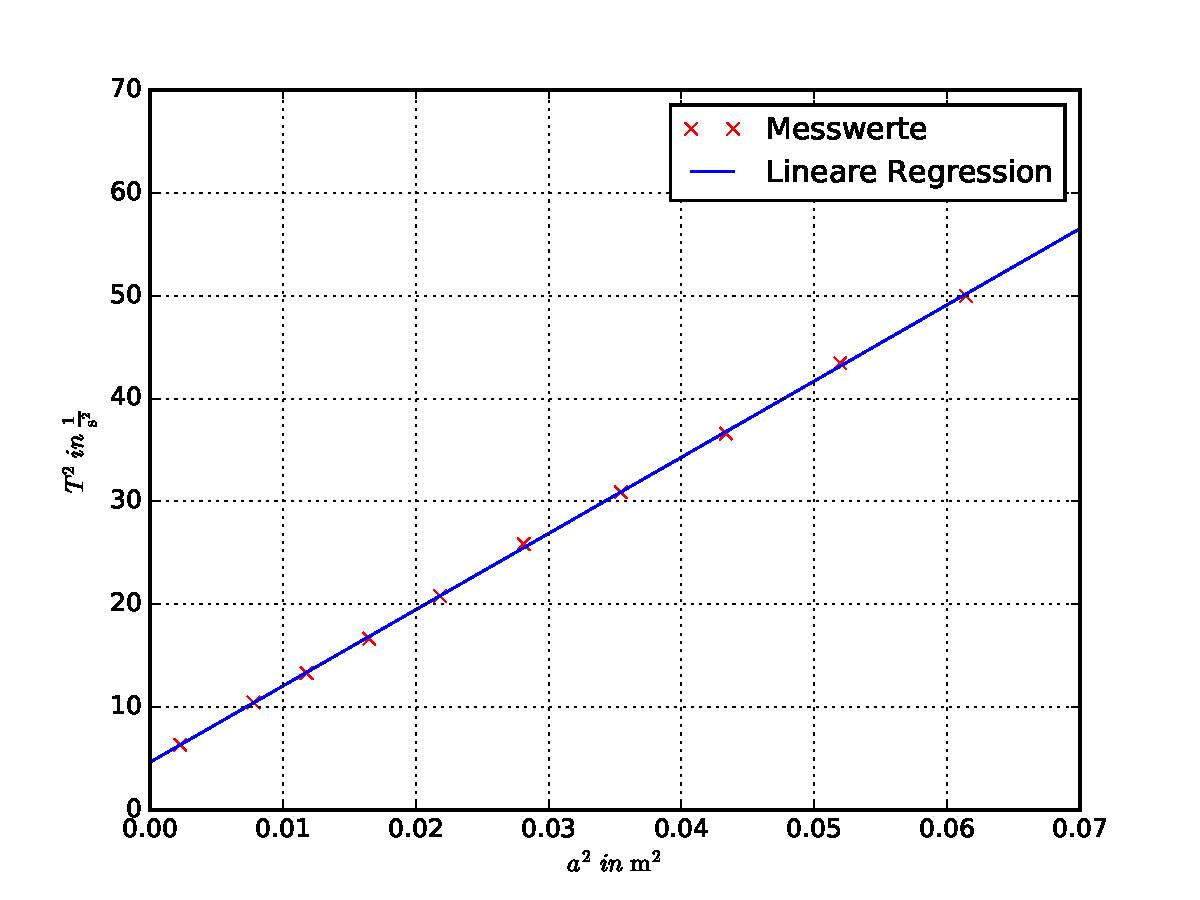
\includegraphics[width=0.9\textwidth]{pics/lineare_regression.pdf}
  \caption{Zusammenhang zwischen $T^2$ und $a^2$}
  \label{fig:zusammenhang_a_T}
\end{figure}

